\section{A Tecnologia de \textit{Web Services}}  \label{cap:ws}

%Unraveling the Web Services Web An Introduction to SOAP, WSDL, and UDDI, 2002
Há alguns anos \deleted{atrás }as aplicações corporativas eram desenvolvidas principalmente em um modelo cliente/servidor de duas camadas, existindo uma aplicação \textit{desktop} que fazia acesso direto a um banco de dados. Pela natureza destas aplicações, que precisam ser instaladas em cada computador onde serão executadas, existe um grande esforço para atualizar todos os computadores com novas versões do sistema. Mesmo que haja um processo automatizado para esta atualização, isto demanda recursos como tempo e largura de banda. Com o avanço das tecnologias de comunicação de dados, o avanço da \textit{Web} e suas linguagens de programação e, principalmente, com o advento da tecnologia AJAX\nomenclature{AJAX}{\textit{Asynchronous Javascript And XML}}, atualmente é possível desenvolver aplicações de \textit{Internet} ricas (\textit{Rich Internet Applications}, RIA\nomenclature{RIA}{\textit{Rich Internet Application}}) com componentes visuais que vão além dos componentes básicos oferecidos pela linguagem HTML\nomenclature{HTML}{\textit{HyperText Markup Language}}. Isto permitiu que muitas empresas migrassem seus sistemas \textit{desktop} para a plataforma \textit{Web}, sem perder funcionalidades existentes naquele tipo de interface.

Essa mudança de paradigma \textit{desktop} para \textit{Web} vem seguida ainda de outra tendência: a dos sistemas distribuídos. 
Estes são sistemas que comumente utilizam a arquitetura cliente/servidor, no entanto, são compostos de três ou mais camadas. 
Segundo \cite{sommerville2011soft}:
\begin{quote}
"um sistema distribuído é uma coleção de computadores independentes que aparece para o usuário como um único sistema coerente."
\end{quote}

A Figura \ref{fig:tree-tiers-app} apresenta uma arquitetura de um sistema distribuído em quatro camadas. As mesmas são descritas a seguir.

\begin{itemize}
	\item Camada de Apresentação: pode contar tanto com aplicações \textit{desktop} leves, conhecidas como \textit{thin client} (cliente magro/leve),
  possuindo apenas uma interface gráfica que faz acesso a um servidor de aplicação, por meio de chamadas de procedimento remoto; quanto com um \textit{browser}, que faz acesso a um servidor \textit{Web}, responsável por gerar as interfaces HTML.
  \item Camada \textit{Web}: composta por um ou mais servidores \textit{Web}, responsáveis por gerar a interface HTML para os clientes \textit{Web}. As aplicações \textit{desktop} não acessam esta camada, tendo ligação direta com a Camada de Aplicação. 
  \item Camada de Aplicação: composta por um ou mais servidores de aplicação onde as regras de negócios da aplicação estão implementadas. Desta forma, alterações na lógica de negócios não requer a atualização dos clientes. Os servidores de aplicação adicionam tolerância a falhas e balanceamento de carga ao sistema.
  \item Camada de Dados: composta por um ou mais servidores de banco de dados, acessíveis apenas pelos servidores de aplicação, o que garante transparência e independência de banco de dados aos clientes.
\end{itemize}

\begin{center}
	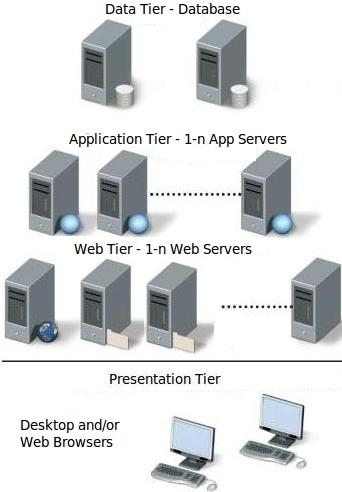
\includegraphics[scale=0.7]{multi-tier-system.png}
	\captionof{figure}{Arquitetura de Aplicação Distribuída (adaptada de \cite{multi-tier-system}).}
	\label{fig:tree-tiers-app}
\end{center}

Segundo \cite{coulouris2007sisdist}, um sistema distribuído traz benefícios como: permitir a heterogeneidade de componentes,
possibilitar a escalabilidade, ser tolerante a falhas, dentre outros.

Neste contexto, \textit{Web Services} (WSs)\nomenclature{WS}{\textit{Web Service}} proveem um \textit{framework} extensível para comunicação de aplicação para aplicação, que utiliza protocolos \textit{Web} existentes e baseados em padrões XML\nomenclature{XML}{\textit{eXtensible Markup Language}} abertos \cite{curbera2002unraveling}. Eles são a maior tecnologia para publicação de serviços na \textit{Web} e têm \replaced{significativa}{significante} adoção em áreas como integração de aplicações, computação distribuída de larga escala e cooperação \textit{business-to-business} (B2B\nomenclature{B2B}{\textit{Business-to-Business}}) \cite{kopecky2008semantic}. Os mesmos são instalados na Camada de Aplicação, como mostrado na Figura \ref{fig:tree-tiers-app}, e proveem um conjunto de padrões para acesso a serviços pela \textit{Internet}, sendo uma tecnologia estabelecida no mercado e cada vez mais adotada por empresas \cite{lausen2007finding}.

\textit{Web Services} permitem o desenvolvimento baseado em componentes, acessíveis por meio da \textit{Internet}. Eles são componentes reutilizáveis, que as aplicações, independentemente da linguagem em que foram implementadas, podem utilizar sem se preocupar em como eles foram desenvolvidos \cite{vilas2007providing}. Desta forma, a construção de aplicações a partir de Web Service segue o processo de desenvolvimento
de \textit{software} conhecido como componentização, como apresentado em \cite{sommerville2011soft}.

Diferentemente de tecnologias como \textit{Common Object Request Broker Architecture} (CORBA)\nomenclature{CORBA}{\textit{Common Object Request Broker Architecture}}, \textit{Distributed Component Object Model} (DCOM)\nomenclature{DCOM}{\textit{Distributed Component Object Model}}, \textit{Component Object Model Plus} (COM+)\nomenclature{COM+}{\textit{Component Object Model Plus}} e 
Java \textit{Remote Method Invocation} (RMI)\nomenclature{RMI}{\textit{Remote Method Invocation}}, WSs usam protocolos \textit{Web} e formatos de dados ubíquos, como HTTP e XML \cite{vilas2007providing}. 

O objetivo dos \textit{Web Services} é alcançar a interoperabilidade entre aplicações, usando padrões \textit{Web}
(\textit{Web standards}). Eles usam um modelo de integração fracamente acoplado para permitir
a integração flexível de sistemas heterogêneos em uma variedade de domínios, 
incluindo \textit{Business-to-Consumer} (\textit{B2C})\nomenclature{B2C}{\textit{Business-to-Consumer}},
\textit{Business-to-Business} (\textit{B2B})
e \textit{Enterprise Application Integration} (\textit{EAI})\nomenclature{EAI}{\textit{Enterprise Application Integration}} \cite{oasis-wsbpel}.


Pela própria natureza distribuída da \textit{Web}, o uso de WSs vem ao encontro da integração entre aplicações heterogêneas, executando em diferentes plataformas, desenvolvidas por diferentes empresas. Cada vez mais empresas disponibilizam serviços, públicos ou privados, para serem utilizados por terceiros, permitindo a interoperabilidade entre diferentes sistemas. Além disto, pelo fato de WSs serem transportados, principalmente, por protocolo HTTP, não sofrem com problemas de portas bloqueadas em \textit{Firewalls} que outras tecnologias, como as mencionadas anteriormente, encontram.
Isto facilita ainda mais a integração entre sistemas hospedados em diferentes redes.

Um \textit{framework} de WSs pode ser dividido em três áreas: protocolos de comunicação,
descrição de serviços e descoberta de serviços \cite{sommerville2011soft}, conforme apresenta 
a Figura \ref{fig:arq-sis-orientados-servicos} e as sub-seções seguintes.

\begin{center}
	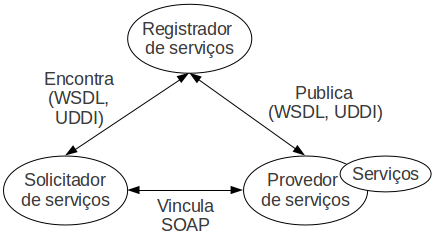
\includegraphics[width=0.7\textwidth]{arq-sis-orientados-servicos.png}
	\captionof{figure}[Arquitetura conceitual de sistemas orientados a serviços]{Arquitetura conceitual de sistemas orientados a serviços (adaptada de \cite{sommerville2011soft}).}
	\label{fig:arq-sis-orientados-servicos}
\end{center}

\subsection{Protocolos de Comunicação}

Dada a natureza distribuída e heterogênea da \textit{Web}, mecanismos de comunicação
devem ser independentes de plataforma, seguros e leves quanto possível.
A linguagem XML é um padrão altamente utilizado para codificação e intercâmbio de dados
entre sistemas, sendo totalmente independente de plataforma. Por esse motivo,
a mesma é utilizada no protocolo de comunicação usado por WSs.

O \textit{Simple Object Access Protocol} (SOAP)\nomenclature{SOAP}{\textit{Simple Object Access Protocol}}, é um protocolo padronizado pelo \textit{World Wide Web Consortium} (W3C),
como protocolo de comunicação para WSs. O SOAP é um protocolo, baseado em XML, para a troca
de mensagens e chamadas de procedimentos remotos (\textit{Remote Procedure Call}, 
RPC\nomenclature{RPC}{\textit{Remote Procedure Call}}). 
No lugar de definir um novo protocolo para empacotar as mensagens, SOAP utiliza protocolos \textit{Web} existentes como HTTP\nomenclature{HTTP}{\textit{HyperText Transfer Protocol}} e SMTP\nomenclature{SMTP}{\textit{Simple Mail Transfer Protocol}}.

Ele é um protocolo leve, adequado para comunicação em um ambiente distribuído e descentralizado \cite{vilas2007providing}.

Uma mensagem SOAP, também denominada "envelope SOAP", é composta por um arquivo XML, contendo um elemento \textit{header} e um \textit{body}.
A Listagem \ref{list:soap-message} mostra a estrutura de um envelope SOAP.

\lstset{caption=Estrutura de um envelope SOAP \cite{curbera2002unraveling}, label=list:soap-message}
\begin{lstlisting}[language=xml]
<SOAP:Envelope 
  xmlns:SOAP="http://schemas.xmlsoap.org/soap/envelope/">
  <SOAP:Header>
      <!-- content of header goes here -->
  </SOAP:Header>

  <SOAP:Body>
      <!-- content of body goes here -->
  </SOAP:Body>
</SOAP:Envelope>
\end{lstlisting}

\subsubsection{Troca de Mensagens SOAP}

Como exemplo para esta seção, vamos utilizar um sistema \textit{Web} de uma companhia aérea, como apresentado em \cite{curbera2002unraveling}.
O sistema disponibiliza um \textit{Web Service} (WS) para a compra de passagens. Uma empresa que vende pacotes turísticos
pode utilizar este WS para integrar o seu sistema com o da companhia aérea,
e assim, fazer todo o processo de registro da passagem dentro do seu próprio sistema.
Desta forma, o sistema da empresa de turismo deve enviar um envelope SOAP
para o WS disponibilizado pela companhia aérea, contendo os dados do cliente
e dados da passagem a ser adquirida, como data/hora, número do voo e do assento 
escolhido pelo cliente. A Listagem \ref{list:http-soap-message} mostra um exemplo
de tal envelope SOAP, empacotado numa mensagem HTTP.

\lstset{caption=Envelope SOAP transportado via HTTP \cite{curbera2002unraveling}, label=list:http-soap-message}
\begin{lstlisting}[language=xml]
POST /travelservice
SOAPAction: "http://www.acme-travel.com/checkin"
Content-Type: text/xml; charset="utf-8"
Content-Length: nnnn

<SOAP:Envelope 
   xmlns:SOAP="http://schemas.xmlsoap.org/soap/envelope/">
   <SOAP:Body>
      <et:eTicket xmlns:et=
         "http://www.acme-travel.com/eticket/schema">
         <et:passengerName first="Joe" last="Smith"/>
         <et:flightInfo airlineName="AA"
              flightNumber="1111"
              departureDate="2002-01-01"
              departureTime="1905"/>
      </et:eTicket>
    </SOAP:Body>
</SOAP:Envelope>
\end{lstlisting}

Observe que o envelope SOAP da Listagem \ref{list:http-soap-message} não possui um \textit{header}.
O mesmo é um elemento opcional e utilizado para prover informações específicas da aplicação,
como credenciais para acesso ao serviço e informações de cobrança, dentre outras\cite{soap-tutorial}.

\subsubsection{Chamadas de Procedimento Remoto Usando SOAP}

Para que SOAP possa usar RPC para chamar procedimentos remotos, é necessário
especificar alguns detalhes para o protocolo RPC, por exemplo:

\begin{itemize}
	\item como valores de tipos são transportados entre  a representação SOAP (XML)
   e a representação da aplicação, e vice-versa (para indicar, por exemplo,
   como deve ser feita a conversão de uma classe Java para XML e vice-versa), e
   \item onde as várias partes do protocolo RPC são transportadas (identificação
   de objeto, nome da operação e parâmetros de entrada e saída).
\end{itemize}

A especificação XML \textit{schema} do W3C \footnote{\url{http://www.w3.org/XML/Schema}} provê uma linguagem padrão
para definir a estrutura do documento e os tipos de dados da estrutura do XML. Isto é,
dado um tipo básico como \textit{integer} ou um tipo complexo como uma \textit{struct}, XML \textit{schema} oferece
uma forma padrão de escrever dados destes tipos em um documento XML. Para habilitar o transporte
de valores tipados, SOAP assume um sistema de tipos baseado em XML \textit{schema}
e define sua codificação em XML. Usando este estilo de codificação pode-se produzir
uma codificação XML para qualquer tipo de dado estruturado.
Parâmetros RPC e retornos são especificados usando esta codificação.

Usando o mesmo WS da companhia aérea, a empresa de turismo
deseja obter informações a respeito de um determinado voo. Assim, seu
sistema pode enviar um envelope SOAP ao WS da companhia aérea.
O envelope da Listagem \ref{list:soap-rpc} mostra uma chamada RPC, encapsulada
dentro de um envelope SOAP. O envelope permite a invocação do método remoto 
\textit{GetFlightInfo}, que recebe dois parâmetros: uma \textit{string} contendo o nome da companhia 
aérea, e um inteiro contendo o número do voo. Tal método retorna um valor estruturado
(uma \textit{struct}) com dois campos: o número do portão de embarque e a situação do voo.

No envelope SOAP, a chamada para \textit{GetFlightInfo} é um elemento XML com atributos
que incluem informações sobre a codificação (note a referência para o XML \textit{schema}). 
Os elementos filhos são os argumentos do método: \textit{airlineName} e \textit{flightNumber}. 
Os tipos são definidos no atributo \textit{type}, onde \textit{xsd} refere-se as definições
de um XML \textit{schema}. Quando o servidor SOAP recebe o envelope, ele converte os valores
\textit{string}, dos atributos \textit{airlineName} e \textit{flightNumber}, para seus
respectivos tipos \textit{string} e inteiro, chamando o método \textit{GetFlightInfo}
passando estes valores.

\lstset{caption=Chamada SOAP RPC empacotada em HTTP \cite{curbera2002unraveling}, label=list:soap-rpc}
\begin{lstlisting}[language=xml]
POST /travelservice
SOAPAction: "http://www.acme-travel.com/flightinfo"
Content-Type: text/xml; charset="utf-8"
Content-Length: nnnn

<SOAP:Envelope 
  xmlns:SOAP="http://schemas.xmlsoap.org/soap/envelope/">
  <SOAP:Body>
    <m:GetFlightInfo
      xmlns:m="http://www.acme-travel.com/flightinfo"
      SOAP:encodingStyle="http://schemas.xmlsoap.org/soap/encoding/"
      xmlns:xsd="http://www.w3.org/2001/XMLSchema"
      xmlns:xsi="http://www.w3.org/2001/XMLSchema-instance">
         <airlineName xsi:type="xsd:string">UL</airlineName>
         <flightNumber xsi:type="xsd:int">506</flightNumber>
    </m:GetFlightInfo>
  </SOAP:Body>
</SOAP:Envelope>
\end{lstlisting}

A Listagem \ref{list:soap-response} mostra a resposta à requisição SOAP enviada
anteriormente. Neste caso, a resposta contém um valor estruturado, com
os campos \textit{gate} (número do portão de embarque) e \textit{status} (situação do voo).

Implementações de SOAP existem para diversas linguagens, como C/C++, Java, Perl e Lua\footnote{Uma implementação
do protocolo SOAP foi feita para uso em aplicações de TV digital desenvolvidas em NCL e Lua, e será apresentada no Capítulo \ref{cap:ncluasoap}.}, que automaticamente geram e processam mensagens SOAP.
Assumindo que as mensagens estão em conformidade com as especificações do protocolo SOAP,
elas podem ser trocadas por serviços implementados em diferentes linguagens e plataformas,
permitindo uma total interoperabilidade entre sistemas heterogêneos, algo que não é sempre
verdade para sistemas que utilizam a arquitetura CORBA, que possui objetivos semelhantes ao SOAP.

\lstset{caption=Resposta de requisição SOAP empacotada em HTTP \cite{curbera2002unraveling}, label=list:soap-response}
\begin{lstlisting}[language=xml]
HTTP/1.1 200 OK
Content-Type: text/xml; charset="utf-8"
Content-Length: nnnn

<SOAP:Envelope 
  xmlns:SOAP="http://schemas.xmlsoap.org/soap/envelope/">
  <SOAP:Body>
    <m:GetFlightInfoResponse 
      xmlns:m="http://www.acme-travel.com/flightinfo"
      SOAP:encodingStyle="http://schemas.xmlsoap.org/soap/encoding/"
      xmlns:xsd="http://www.w3.org/2001/XMLSchema"
      xmlns:xsi="http://www.w3.org/2001/XMLSchema-instance">
         <flightInfo>
           <gate xsi:type="xsd:int">10</gate>
           <status xsi:type="xsd:string">ON TIME</status>
         </flightInfo>
     </m:GetFlightInfoResponse>
   </SOAP:Body>
</SOAP:Envelope>
\end{lstlisting}

\subsection{Descrição de Serviços}

O protocolo SOAP define uma linguagem padrão para uso de WSs,
mas ele não informa quais mensagens devem ser trocadas para 
que tenhamos sucesso no uso de um determinado serviço.
Para isto, existe a \textit{Web Service Description Language} (WSDL)\nomenclature{WSDL}{\textit{Web Service Description Language}}, 
uma linguagem também baseada em XML. Um documento WSDL descreve
a interface de um WS, permitindo que as aplicações
que consumirão o serviço disponibilizado, saibam quais informações
devem incluir dentro de um envelope SOAP. Desta forma, podem chamar
um determinado procedimento remoto disponibilizado pelo WS.
O WSDL descreve um WS como uma coleção de \textit{end points}
que podem trocar certas mensagens \cite{curbera2002unraveling}. Um \textit{end point} é um
elemento no WSDL que define a ligação entre a definição de um 
determinado serviço e o seu endereço de rede, permitindo o acesso
ao mesmo.

As mensagens SOAP anteriormente mostradas não poderiam ter sido
construídas se não conhecêssemos o documento WSDL que descreve
o serviço que desejamos utilizar. Informações
como o nome do método a ser acessado e o nome e tipos dos parâmetros
de entrada e saída foram obtidos a partir do WSDL do serviço \cite{curbera2002unraveling}.

Um serviço completo de descrição WSDL provê dois pedaços de informação:
uma descrição do serviço em nível de aplicação, ou interface abstrata, e 
detalhes específicos dependentes do protocolo, que os usuários
devem seguir para acessar o serviço em \textit{end points} concretos \cite{curbera2002unraveling}.

\subsubsection{Descrição de um \textit{Web Service}}

Um documento WSDL define uma descrição abstrata de um serviço, em termos
de troca de mensagens em uma interação com o mesmo. Existem três principais
componentes desta interface abstrata: o vocabulário, a mensagem e a interação. 
Acordo para uso de um determinado vocabulário é a fundação para qualquer tipo
de comunicação. Um WSDL usa sistemas de tipos externos para prover definição
de tipos de dados para troca de informações. Embora o WSDL possa suportar
qualquer sistema de tipos, a maioria dos serviços usa o XML \textit{Schema Definition} (XSD)\nomenclature{XSD}{\textit{XML Schema Definition}}.
Na Listagem \ref{list:wsdl-description}, podemos ver o uso de dois tipos 
de dados definidos no XSD (\textit{int} e \textit{string}), e dois tipos de dados definidos
em um \textit{schema} externo (\textit{FlightInfoType} e \textit{Ticket}).
O WSDL pode importar tais definições XSD externas usando um elemento 
\textit{import}, especificando sua localização \cite{curbera2002unraveling}.

O WSDL define elementos \textit{message} contendo partes, cada qual descrita
por tipos XSD ou elementos de um vocabulário pré-definido.
Cada \textit{message} provê uma definição de dados tipados e abstratos
enviados e recebidos pelos serviços. Uma mensagem pode ser de entrada (\textit{input}),
definindo o tipo do(s) parâmetro(s) que uma determinada função deve receber; 
ou de saída (\textit{output}), indicando o(s) tipo(s) de valor(es) a ser(em) retornado(s)
pela função, como pode ser visto na Listagem \ref{list:wsdl-description} \cite{curbera2002unraveling}.

Os elementos \textit{portType} e \textit{operation} combinam mensagens para definir
iterações. Cada \textit{operation} representa um padrão de troca de mensagens
suportado pelo WS. Cada \textit{operation} é uma combinação de mensagens
rotuladas como \textit{input} (entrada), \textit{output} (saída) ou \textit{fault} (falha),
para indicar o papel de cada mensagem em uma iteração \cite{curbera2002unraveling}.

Um \textit{portType} é uma coleção de operações que são coletivamente suportadas
por um \textit{end point} (\textit{port}). No exemplo da Listagem \ref{list:wsdl-description},
\textit{AirportServicePortType} descreve duas operações: uma única operação
no estilo \textit{request-response}, \textit{GetFlightInfo}, que espera
uma mensagem \textit{GetFlightInfoInput} como entrada e retorna
uma mensagem \textit{GetFlightInfoOutput} como resposta; e uma operação
uni direcional, \textit{CheckIn}, que apenas recebe uma mensagem \textit{CheckInInput}
como entrada \cite{curbera2002unraveling}.

\lstset{caption=Fragmento de uma descrição de WSDL \cite{curbera2002unraveling}, label=list:wsdl-description}
\begin{lstlisting}[language=xml]
<message name="GetFlightInfoInput">
  <part name="airlineName" type="xsd:string"/>
  <part name="flightNumber" type="xsd:int"/>
</message>

<message name="GetFlightInfoOutput">
  <part name="flightInfo" type="fixsd:FlightInfoType"/>
</message>

<message name="CheckInInput">
  <part name="body" element="eticketxsd:Ticket"/>
</message>

<portType name="AirportServicePortType">
  <operation name="GetFlightInfo">
    <input message="tns:GetFlightInfoInput"/>                   
    <output message="tns:GetFlightInfoOutput"/>
  </operation>
  <operation name="CheckIn">
    <input message="tns:CheckInInput"/>
</operation>
</portType>
\end{lstlisting}

\subsubsection{Informações de \textit{Binding}}

A especificação do WSDL apresenta três tipos de informações sobre
o serviço\cite{sommerville2011soft}:

\begin{itemize}
	\item quais operações o serviço suporta (chamado de interface);
  \item como mapear as interfaces abstratas para um conjunto de protocolos concretos (\textit{binding}), e
  \item onde está a implementação dos métodos suportados pelo serviço (o endereço de rede).
\end{itemize}


Por meio do \textit{binding} temos a resposta para o "como",
incluindo o protocolo de comunicação e especificação de formato de dados
para um completo elemento \textit{portType}. Sucintamente, o elemento \textit{binding}
diz como dada interação ocorre sobre o protocolo especificado. A Listagem \ref{list:wsdl-binding}
mostra um fragmento para o exemplo citado. O \textit{binding} descreve como usar SOAP
para acessar o serviço \textit{travelservice}. Em particular, o documento WSDL mostra que:

\begin{itemize}
	\item \textit{GetFlightInfo} usará interações em estilo SOAP-RPC,
  em que todas as trocas de mensagens usam codificação padrão SOAP, e
  \item \textit{CheckIn} é uma interação de mensagem pura (chamada de orientada a documento
  em termos de WSDL), em que o corpo do envelope SOAP contém a mensagem codificada,
  sem nenhuma codificação de tipo adicional; isto é, ele usa XSD para literalmente descrever
  o XML transmitido.
\end{itemize}

O restante do documento descreve o "onde", para ligar a interface abstrata, protocolo
e detalhes de \textit{marshalling}\footnote{Processo de organizar dados em computador, de forma padronizada,
para permitir que diferentes aplicações possam utilizar tais dados, garantindo
a interoperabilidade.}, promovendo a ligação (\textit{binding}) desses elementos para permitir
o acesso aos métodos do serviço. Um elemento \textit{port} descreve um único \textit{end point}
como uma combinação de um \textit{binding} e um endereço de rede. Consequentemente, um elemento
\textit{service} pode agrupar um conjunto de \textit{ports} relacionados.

\lstset{caption=Informações concretas de ligação em um WSDL \cite{curbera2002unraveling}, label=list:wsdl-binding}
\begin{lstlisting}[language=xml]
<binding name="AirportServiceSoapBinding"
  type="tns:AirportServicePortType">
  <soap:binding 
     transport="http://schemas.xmlsoap.org/soap/http"/>
  <operation name="GetFlightInfo">
    <soap:operation style="rpc"
          soapAction="http://acme-travel/flightinfo"/>
    <input>
      <soap:body use="encoded"
          namespace="http://acme-travel.com/flightinfo"
          encodingStyle=
           "http://schemas.xmlsoap.org/soap/encoding/"/>
    </input>
    <output>
      <soap:body use="encoded"
          namespace="http://acme-travel.com/flightinfo"
          encodingStyle=
           "http://schemas.xmlsoap.org/soap/encoding/"/>
    </output>
  </operation>

  <operation name="CheckIn">
    <soap:operation style="document"
          soapAction="http://acme-travel.com/checkin"/>
    <input>
      <soap:body use="literal"/>
    </input>
  </operation>
</binding>

<service name="travelservice">
  <port name="travelservicePort"
     binding="tns:AirportServiceSoapBinding">
  <soap:address 
     location="http://acmetravel.com/travelservice"/>
  </port>
</service>
\end{lstlisting}

A Figura \ref{fig:wsdl-organization} mostra como a especificação do WSDL é organizada.
A seção \textit{Introdução} do WSDL contém a declaração dos \textit{Namespaces} XML contendo as definições
de tipos padrões usados pelo \textit{Web Service}. A seção \textit{Interface Abstrata}
apresenta os tipos definidos pelo \textit{Web Service}, as declarações de interfaces (os \textit{portTypes})
e as mensagens suportadas (como mensagens com os parâmetros de entrada a serem enviadas a um método no \textit{Web Service}
e as mensagens de saída com o retorno do método).
A seção \textit{Implementação Concreta} contém as informações de \textit{binding} (como o protocolo a
ser utilizado na troca de mensagens) e os \textit{end points} (as interfaces
concretas para realização da vinculação da aplicação cliente com o endereço de rede do \textit{Web Service}.

\begin{center}
	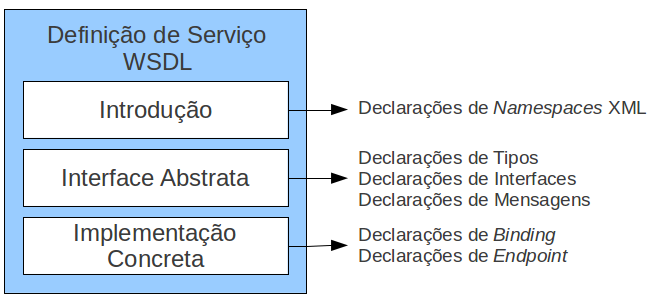
\includegraphics[width=0.80\textwidth]{wsdl-organization.png}
	\captionof{figure}[Organização da Especificação do WSDL]{\added{Organização da Especificação do WSDL\cite{sommerville2011soft}.}}
	\label{fig:wsdl-organization}
\end{center}



\subsubsection{Usando o WSDL}

Para usuários e desenvolvedores, o WSDL provê uma descrição formal das interações cliente/servidor.
Desenvolvedores podem usar o documento WSDL como entrada para uma aplicação que gere 
funções \textit{proxy}\footnote{Tais funções \textit{proxy} são escritas ou geradas
na linguagem utilizada pela aplicação cliente (que consome o \textit{Web Service}). Elas possuem
a mesma assinatura dos métodos remotos, tornando transparente para o cliente a chamada
aos métodos no WS. São responsáveis por gerar o envelope SOAP para enviar ao
servidor onde o WS é hospedado.},
utilizadas no cliente, para acesso aos métodos do WS. Tais funções \textit{proxy}
também podem ser geradas dinamicamente, em tempo de execução, por rotinas implementadas
no cliente que interpretam o WSDL e geram as chamadas SOAP necessárias.
Em ambos os casos, as funções \textit{proxy} têm a finalidade de esconder do cliente toda a complexidade
envolvida no processo de chamada dos métodos remotos.

\subsection{Descoberta de Serviços com UDDI} \label{sec:uddi}

As especificações do \textit{Universal Description, Discovery and Integration} (UDDI)\nomenclature{UDDI}{\textit{Universal Description, Discovery and Integration}} oferecem aos usuários uma forma sistemática e unificada para encontrar provedores
de serviços através de um registro centralizado de serviços, que é, grosseiramente,
equivalente a uma "lista telefônica" \textit{online} de WSs \cite{curbera2002unraveling}.
O \textit{UDDI Business Registry} (UBR)\nomenclature{UBR}{\textit{UDDI Business Registry}}, acessível por meio de um \textit{browser}, foi
disponibilizado pouco tempo após a especificação se tornar pública, no entanto, o mesmo foi descontinuado
em 2005\footnote{\url{http://uddi.microsoft.com/about/FAQshutdown.htm}} \cite{treiber2007active}.

Segundo \cite{sommerville2011soft}, o padrão UDDI não foi amplamente adotado.
UDDI provê dois tipos básicos de especificação que definem a estrutura
e operação do registro de serviços \cite{curbera2002unraveling}:

\begin{itemize}
	\item uma definição da informação para prover sobre cada serviço, e como codificá-la; e
  \item uma API\nomenclature{API}{\textit{Application Programming Interface}} de busca e atualização para o registro, que descreve como esta informação
  pode ser acessada e atualizada.
\end{itemize}

O acesso ao registro é realizado usando uma API SOAP para busca e atualização. 

\begin{comment}
\subsubsection{Estrutura do UDDI}

O UDDI codifica três tipos de informações sobre \textit{Web Services}:

\begin{itemize}
	\item informações de \textbf{páginas brancas} incluem nome e detalhes de contato;
  \item informações de \textbf{páginas amarelas} proveem uma categorização baseada em tipos
  de negócio e serviço; e
  \item informações de \textbf{páginas verdes} incluem dados técnicos sobre o serviço.
\end{itemize}

O registro UDDI é organizado ao redor de duas entidades fundamentais que descrevem negócios e os serviços que eles proveem. O elemento \textit{businessEntity} (entidade de negócio), apresentado na Listagem \ref{list:uddi-businessEntity}, provê informações padrões de "páginas brancas", incluindo identificadores (como CPF/CNPJ), informações de contato e uma descrição simples. Cada entidade de negócio deve incluir deve incluir um ou mais elementos \textit{businessServices} (serviço de negócio), mostrado na Listagem \ref{list:uddi-businessService}, que representam os serviços que ele provê. Ambas elementos de negócio e serviço podem especificar um elemento \textit{categoryBag} para categorizar o negócio ou serviço (que será discutido adiante).

\lstset{caption=Estrutura simplificada do \textit{businessEntity} de um serviço no UDDI \cite{curbera2002unraveling}, label=list:uddi-businessEntity}
\begin{lstlisting}[language=xml]
<businessEntity businessKey=
       "A687FG00-56NM-EFT1-3456-098765432124">
 <name>Acme Travel Incorporated</name>
 <description xml:lang="en">
   Acme is a world leader in online travel services
 </description>
 <contacts>
   <contact useType="US general">
     <personName>Acme Inc.</personName>
     <phone>1 800 CALL ACME</phone>
     <email useType="">acme@acme-travel.com</email>
     <address>
       <addressLine>Acme</addressLine>
       <addressLine>12 Maple Avenue</addressLine>
       <addressLine>Springfield, CT 06785</addressLine>
     </address>
   </contact>
 </contacts>
 <businessServices> ...
 </businessServices>
 <identifierBag> ...
 </identifierBag>
 <categoryBag> ...
   <keyedReference tModelKey=
         "UUID:DB77450D-9FA8-45D4-A7BC-04411D14E384"
         keyName="Electronic check-in"
         keyValue="84121801"/>
 </categoryBag>
</businessEntity>
\end{lstlisting}

As Listagens \ref{list:uddi-businessEntity} e \ref{list:uddi-businessService} mostram um importante aspecto do projeto de UDDI: chaves únicas identificam cada entidade de dados - negócios, serviços e tudo mais - que podem referenciar umas as outras. Estas chaves são \textit{strings} hexadecimais geradas quando a entidade (neste caso, o negócio) é registrada. As chaves são identificadores universalmente únicos (\textit{Universally Unique Identifiers}, UUIDs). Por exemplo, o atributo \textit{businessKey} (chave de negócio) identifica um negócio unicamentee um atributo \textit{serviceKey} (chave de serviço) identifica unicamente um serviço. Um serviço também referencia seu host pela sua \textit{businessKey}. Em adição a informações inteligíveis como descrição, nome e categorização, a entidade \textit{service} contém uma lista de \textit{bindingTemplates}, que codificam informações técnicas de acesso ao serviço. Cada \textit{bindingTemplate} representa um ponto de acesso ao serviço, indicando que o serviço pode ser acessado de diferentes \textit{end points}.

\lstset{caption=Estrutura simplificada do \textit{businessService} de um serviço no UDDI \cite{curbera2002unraveling}, label=list:uddi-businessService}
\begin{lstlisting}[language=xml]
<businessService serviceKey=
      "894B5100-3AAF-11D5-80DC-002035229C64"
    businessKey=
      "D2033110-3AAF-11D5-80DC-002035229C64">
  <name>ElectronicTravelService</name>
  <description xml:lang="en">Electronic Travel Service</description>
  <bindingTemplates>
    <bindingTemplate bindingKey=
          "6D665B10-3AAF-11D5-80DC-002035229C64"
        serviceKey=
          "89470B40-3AAF-11D5-80DC-002035229C64">
      <description>
        SOAP-based e-checkin and flight info
      </description>
      <accesssPoint URLType="http">
        http://www.acme-travel.com/travelservice
      </accessPoint>
      <tModelInstanceDetails>
        <tModelInstanceInfo tModelKey=
          "D2033110-3BGF-1KJH-234C-09873909802">
        ...
        </tModelInstanceInfo>
      </tModelInstanceDetails>
    </bindingTemplate>
  </bindingTemplates>
  <categoryBag> ...
  </categoryBag>
</businessService>
\end{lstlisting}

\subsubsection{Descrição Técnica e tModels}
...

\subsubsection{Categorização}

Localizar particulares tipos de negócios e serviços eficientemente depende da nossa habilidade de qualificar as entradas de negócios e serviços no diretório, de acordo com um esquema de categorização ou taxonomia, usando informações como localização geográfica, tipo de indústria ou produto, para caracterizar o serviço.

Para identificar sistemas de taxonomia, cada sistema de classificação é registrado com um \textit{tModel} no registro UDDI. Informações taxonômicas são então codificadas em pares de nome-valor, qualificados por uma referência a uma chave de um \textit{tModel}, que identifica a qual taxonomia cada par pertence. Três taxonomias padrões são citadas pelo UDDI e pré-registradas no UBR:

\begin{itemize}
	\item uma classificação de indústria, obedecendo à taxonomia do \textit{North American Industry Classification System},NAICS (Sistema de Classificação Industrial Norte Americano)\nomenclature{NAICS}{\textit{North American Industry Classification System}};
  \item uma classificação de produtos e serviços obedecendo à taxonomia do \textit{Universal Standard Products and Services Code System} (USPSCS) (Padrão Universal de Sistema de Código de Produtos e Serviços)\nomenclature{USPSCS}{\textit{Universal Standard Products and Services Code System}}; e
  \item um sistema de categorização geográfica obedecendo à taxonomia do \textit{International Organization for Standardization Geographic} (ISO 3166\footnote{Um padrão de identificação de países, que possui tanto códigos alfabéticos no formato de 2 e 3 letras, quanto códigos numéricos de 3 dígitos. Os códigos para o Brasil, por exemplo, podem ser BR, BRA ou 076.}).\nomenclature{ISO}{\textit{International Organization for Standardization}}
\end{itemize}

Usando categorização, podemos pesquisar no diretório UDDI por tipos de serviços específicos. Um vez encontrado o serviço, podemos obter sua descrição WSDL para saber como utilizá-lo.
\end{comment}

\subsection{\textit{Web Services} REST}

Como visto anteriormente, SOAP é o padrão W3C para \textit{Web Services}, amplamente utilizado
na integração de aplicações heterogêneas. No entanto, existe uma outra vertente para construção de \textit{Web Services}
denominada REST. O REST é o acrônimo para \textit{Representational State Transfer}\nomenclature{REST}{\textit{Representational State Transfer}}. 
Ele é um estilo arquitetural para construção de aplicações distribuídas que também permite a integração de aplicações heterogêneas,
mas não é um padrão W3C.

O estilo REST foi apresentado pela primeira vez no trabalho de dissertação de Roy Fielding\cite{fielding2000architectural},
sendo baseado em padrões \textit{Web} como HTTP e URL. Ele consiste em prover serviços \textit{Web}
a partir de um recurso \textit{Web} acessível por meio de uma URL\nomenclature{URL}{\textit{Uniform Resource Locator}}. 
A interação com tal serviço é feita por meio de uso dos métodos HTTP como \textit{GET}, \textit{POST} e \textit{DELETE} para passagem de parâmetros ao serviço.
Tal estilo é bastante simplificado em relação ao SOAP, pois todos os dados a serem passados ao serviço
vão diretamente na URL do mesmo, por meio de uma requisição HTTP. Desta forma, o tamanho de uma requisição REST
é bastante reduzido em relação ao SOAP.

REST não define um padrão de formato das mensagens de resposta, no entanto, pode-se perfeitamente utilizar
XML para isto. Atualmente outros padrões de formato de dados são bastante utilizados como o \textit{JavaScript Object Notation} (JSON)\nomenclature{JSON}{\textit{JavaScript Object Notation}}. Desta forma, pode-se utilizar qualquer padrão que se desejar, como por exemplo,
o formato de dados definido pela linguagem Lua, sendo bastante útil em aplicações para o Sistema Brasileiro de TV Digital, desenvolvidas em tal  linguagem, por utilizar um formato nativo da mesma.

O estilo REST atualmente se tornou um padrão de fato e é amplamente utilizado para integração
de serviços \textit{Web} com aplicações de diferentes tipos, como é o caso dos serviços disponibilizados
pelo \textit{microblog Twitter}. Este permite que desenvolvedores construam aplicações 
nas mais diferentes plataformas (\textit{Web, desktop, mobile}) que se integrem
com o serviço de \textit{microblog}.

O REST também segue a arquitetura cliente/servidor usada no protocolo SOAP. 
Segundo \cite{welling2006integration}, o estilo é denominado REST (em português, Transferência de Estado Representacional), pois o cliente obtém
uma representação de um recurso através de uma URL, o que faz com que a aplicação cliente
entre em um determinado estado. O cliente pode selecionar um link que foi incluído no primeiro recurso para,
por exemplo, obter informações detalhadas. Como o link direciona para outro recurso, a aplicação cliente
obtém uma nova representação de um recurso e entra em um novo estado.

Como citado, a grande vantagem do REST é sua simplicidade, no entanto, 
por não haver um padrão de passagem de parâmetros e formato de dados
para a respostas das requisições, tal estilo pode não ser adequado para 
a construção de aplicações seguindo o padrão de arquitetura orientada
a serviços, onde uma aplicação pode utilizar serviços de diferentes provedores.
Usando REST, cada provedor de serviços pode definir sua forma de passar os parâmetros
e o formato de dados da mensagem de retorno, assim a aplicação que integra com todos
os provedores precisará implementar diversos formatos de entrada e saída de dados.
Com o SOAP isto não ocorre, pois todos os provedores seguem um padrão bem definido
e a aplicação cliente implementa apenas tal padrão.

\subsection{Arquitetura Orientada a Serviços}

Segundo \cite{sommerville2011soft}, uma arquitetura orientada a serviços (\textit{Service Oriented Architecture} - SOA)
é uma forma de desenvolvimento de sistemas distribuídos onde os componentes de tal sistema são serviços \textit{stand-alone} (autônomos),
executando em computadores geograficamente distribuídos. Em tal arquitetura, ainda segundo \cite{sommerville2011soft}, 
usar \textit{Web Services} é uma forma de as organizações tornarem suas informações acessíveis. Com isto, é possível
haver a integração entre empresas, mesmo que por meio de sistemas heterogênos completamente diferentes.

